\chapter[~~~CONCEPTION]{~~~II -~Conception de l’application}%
\label{refDev2}%

Ce chapitre explique la conception de l'application \nom\~et les choix réalisés pour sa réalisation. Il détaille les diagrammes de classes, les structures de données et les algorithmes intéressants.

\section{Diagramme de classes}

Cette section présente le diagramme de classes du projet \nom. Il est composé de plusieurs classes et interfaces.
% \bigskip

\begin{figure}[!ht] 
  \centering% 
  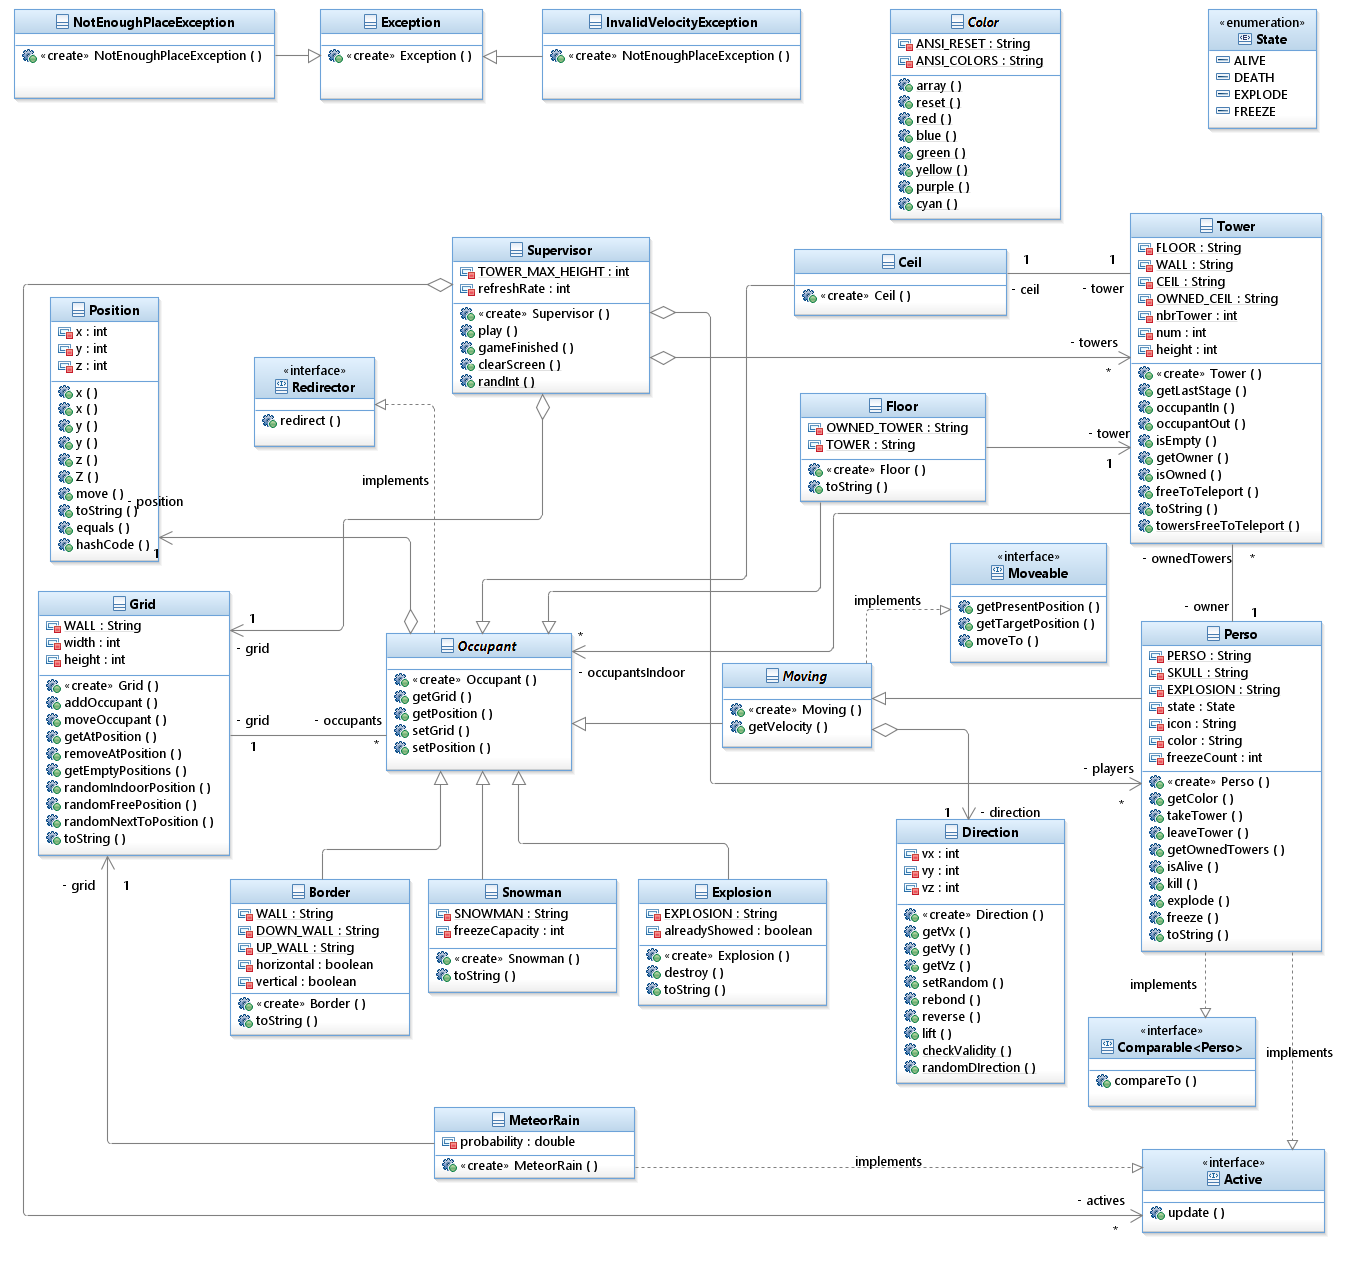
\includegraphics[width=13.9cm]{assets/pictures/ToursInfernales_Main.png}% 
  \caption{Diagramme de classes complet du projet}%
  %\label{Q1}
\end{figure}
\newpage

\section{Choix des structures de données}

Le projet \nom\~utilise plusieurs structures de données pour stocker les informations des personnages, des murs et des tours:

\begin{itemize}
    \item \emph{HashMap} $\rightarrow$ Utilisée dans la grille pour stocker les occupants tout en ayant accès à leur position en indice.
    \item \emph{List} $\rightarrow$ Utilisée notamment dans les choix aléatoires. La première structure détermine les choix possibles et la second utilise la méthode \emph{get} pour sélectionner avec un indice choisit aléatoirement. Implémentée en tant que \emph{ArrayList}.
    \item \emph{Set} $\rightarrow$ Utilisée pour renvoyer un ensemble d'objets dont le seul besoin et de parcourir la collection du début à la fin à l'aide d'un \emph{foreach}. Implémentée en tant que \emph{HashSet}.
    \item \emph{Queue} $\rightarrow$ Implémentée en tant que \emph{PriorityQueue} dans le superviseur pour déterminer l'ordre du classement des personnages.
\end{itemize}

\section{Algorithmes intéressants}

Cette section présente les algorithmes intéressants utilisés dans le projet \nom.

\subsection{Algorithme de détermination du classement final}

Dans un premier temps nous allons présenté un algorithme intéressant utilisé dans le projet \nom~. Il s'agit de l'algorithme de détermination du classement final des personnages. Cet algorithme est utilisé dans la méthode \emph{play} de la classe \emph{Supervisor} pour déterminer le classement final des personnages en fonction de leur score. 

L'algorithme utilise un tri par tas pour déterminer l'ordre du classement. On entasse puis destasse ce qui a pour effet de trier les éléments en fonction de leur priorité déterminée par la méthode \emph{compareTo}. L'algorithme est présenté dans l'encadré ci-dessous. Nous n'avons pas utiliser pour cela la méthode \emph{sort} de la classe \emph{Collections} par préférence personnel car nous n'avons pas connaissance de l'exactitude de l'algorithme utilisé dans \emph{sort}.


%%% algo 
\begin{algorithm}
\caption[\emph{Algorithme de détermination du classement final}]{\label{algo}Algorithme de détermination du classement final.}

public Perso[] play\?(int maxRound) throws InterruptedException \tab{}{
  
\dots
\bigskip


// get and return players in order using heap sort

Queue<Perso> heap = new PriorityQueue<Perso>\?();

for (Perso player: this.players) \tab{}{
  heap.add\?(player);
}

for (int i=this.players.length-1; i >= 0; i--) \tab{}{
  this.players[i] = heap.poll\?();
}

return this.players;
}
\end{algorithm}
\bigskip


\subsection{Algorithme de la pluie de météorites}

Dans un second temps nous allons présenté l'algorithme de la pluie de météorites. Cet algorithme est utilisé dans la méthode \emph{update} de la classe \emph{MeteorRain} pour déterminer si une météorite doit être lancée ou non. Il se base sur l'attribut \emph{probqbility} de la classe pour choisir avec plus ou moins de probabilité si une météorite doit être lancée ou non. Si la météorite lancée touche un personnage, elle le tue avec la méthode adaptée, sinon si la case est vide un simple spite d'explosion apparait avec une frame de durée de vie. L'algorithme est présenté dans l'encadré ci-dessous.

%%% algo 
\begin{algorithm}
  \caption[\emph{Algorithme de la pluie de météorites}]{\label{algo2}Algorithme de la pluie de météorites.}

  @Override

  public void update\?() \tab{}{
    // launch a meteor or not

    if (Math.random\?() <= this.probability) \tab{}{
      // choose a random cell and get it

      Position pos = this.grid.randomIndoorPosition\?();

      Occupant target = this.grid.getAtPosition\?(pos);

      // explode the player if it exists

      if (target instanceof Perso) \tab{}{
        Perso player = (Perso)\?target;

        if (player.isAlive\?()) \tab{}{
          player.explode\?();
        }
      }
      else if (target == null) \tab{}{
        new Explosion\?(this.grid, pos);
      }
    }
  }
\end{algorithm}